\section{Clock 2: training as a dynamical system}
\label{sec:clock2}

\subsection{Gradient descent at the edge of stability}
\label{sec:eos}

Classical optimization theory treats gradient descent as a discretization of gradient flow, which is valid when the step size is small compared with the inverse curvature. \citet{cohen2021gradient} showed that neural network training does not stay in that regime. Under full-batch gradient descent the sharpness, meaning the largest Hessian eigenvalue $\lambda_{\max}$, first rises (progressive sharpening) until it reaches $2/\eta$, and then hovers near that value while the loss keeps decreasing in a non-monotone way. By the linear stability argument of Section~\ref{sec:tools}, the iteration then sits on the boundary where the top direction loses stability. Adaptive methods show the same behavior with respect to the preconditioned sharpness \citep{cohen2022adaptive}.

Several mechanisms have been proposed for why training survives at this boundary. \citet{damian2022selfstabilization} show that the third-order term of the loss creates a negative feedback: when the iterate oscillates along the top eigenvector, the oscillation itself reduces the sharpness. In their reduced model, $x_t$ is the displacement along the top eigenvector $u$ and $y_t$ is the excess of the sharpness over $2/\eta$, measured along $\nabla S$, and the two evolve as
\begin{equation}
x_{t+1}=-(1+\eta y_t)\,x_t,\qquad y_{t+1}=y_t+\eta\big(\alpha-\beta x_t^2\big),
\label{eq:selfstab}
\end{equation}
where $\alpha>0$ measures progressive sharpening and $\beta=\|\nabla S\|^2$. The oscillation grows while $y_t>0$ and its square pulls $y_t$ back, so the pair cycles around the edge instead of diverging. \citet{arora2022gradient} and \citet{ahn2022unstable} give conditions under which gradient descent converges while being locally unstable. Minimal models help because they can be solved: \citet{zhu2022edgeofstability} find edge-of-stability dynamics in a two-parameter example, and \citet{chen2022edge} show that beyond the threshold gradient descent can converge to stable period-two orbits, a period-doubling bifurcation in the strict sense. Backward error analysis of the finite step shows that gradient descent follows a modified flow with an implicit penalty on the gradient norm \citep{barrett2020implicit}.

Larger step sizes push the map further. \citet{lewkowycz2020large} identified a catapult phase in which the loss first grows, the curvature drops, and training settles in a flatter region; above a second threshold training diverges. \citet{kalra2023phase} mapped the early-training regimes as a function of learning rate, depth and width. \citet{kong2020stochasticity} showed that deterministic gradient descent on a multiscale objective, with a step size that resolves only the macroscopic scale, can become chaotic and converge to a statistical distribution. \citet{tuci2026generalization} model stochastic optimizers at the edge of stability as random dynamical systems with fractal attractors and relate the attractor dimension to generalization. \citet{sohldickstein2024boundary} found that the boundary in hyperparameter space between step sizes that train and those that diverge is fractal, in the same way as the boundary of bounded orbits of the quadratic map that defines the Mandelbrot set. Mini-batch sampling moves this stability boundary even when gradients are unbiased, as shown exactly for linear self-attention \citep{balasubramanian2026unbiased}. Curvature control has been used to keep large transformers away from the boundary \citep{ramasinghe2026taming,gilmer2021loss}.

A continuous-time description of the whole edge-of-stability regime is now available. The central flow of \citet{cohen2024central} is an ODE for the time-averaged trajectory that keeps the sharpness at $2/\eta$ and predicts the loss curve of real networks, and \citet{berthier2026multiple} derives it by a formal expansion in three time scales with the method of multiple scales. \citet{marion2026edge} proposes a related three-variable flow for the center, direction and amplitude of the oscillation. Bifurcation theory gives the local picture. \citet{song2023trajectory} prove that in simple models trajectories align on a bifurcation diagram, \citet{gan2026bifurcation} treats the onset of oscillation as a flip bifurcation of the normal dynamics near a manifold of minimizers, and \citet{mulayoff2026stability} give an exact criterion, in terms of third and fourth derivatives, for when oscillations near a minimum are stable. \citet{litman2026origin} shows that a weighted average of the curvature along the steps is forced to $2/\eta$. Why the sharpness rises in the first place, progressive sharpening, is proved only in reduced models \citep{agarwala2022secondorder}, and the route from the edge to chaos at larger steps has been mapped in a two-layer linear model \citep{kalra2023universal}. Section~\ref{sec:exp2} adds a measurement to this picture: in a small transformer the edge is multi-mode, with several eigenvalues above $2/\eta$, while the curvature along the step equals $2/\eta$.

\subsection{Stochastic gradient descent as a noisy dynamical system}
\label{sec:sgd}

Minibatch noise turns clock~2 into a stochastic process. Stochastic modified equations approximate SGD with step size $\eta$ and batch size $B$ by the SDE
\begin{equation}
d\theta=-\nabla\mathcal{L}(\theta)\,dt+\sqrt{\tfrac{\eta}{B}\,C(\theta)}\;dW_t ,
\label{eq:sme}
\end{equation}
where $C$ is the covariance of per-example gradients and time is measured in units of $\eta$ \citep{li2015stochastic}. Near a minimum with Hessian $H$ the drift is linear, the process is of Ornstein-Uhlenbeck type, and its stationary covariance $\Sigma$ solves the Lyapunov equation $H\Sigma+\Sigma H=(\eta/B)\,C$, so the ratio $\eta/B$ acts as a temperature \citep{mandt2017stochastic,smith2017bayesian,jastrzebski2017three}. Because SGD noise is anisotropic and state dependent, the stationary distribution is not a Gibbs distribution of the training loss, and the dynamics can converge to limit cycles instead of points \citep{chaudhari2017stochastic}.

Escape from a minimum is the most direct use of the escape theory sketched in Section~\ref{sec:tools}. \citet{xie2020diffusion} derived a Kramers-type rate for SGD and found that, unlike isotropic Langevin dynamics, SGD favors flat minima exponentially in the ratio of barrier height to Hessian eigenvalues. Anisotropic noise aligned with the curvature helps escape from sharp minima \citep{zhu2018anisotropic}. \citet{mori2021powerlaw} showed that the multiplicative character of the noise changes the law: the escape rate depends on the logarithm of the loss barrier, which gives an escape rate that scales as a power of the loss ratio between saddle and minimum. Heavy-tailed gradient noise points toward L\'evy-driven escape, which is dominated by single large jumps \citep{simsekli2019tailindex}. The precise law therefore depends on the noise model, and the law that holds for language model pretraining has not been measured.

\subsection{Saddles, plateaus and ghosts}

High-dimensional loss surfaces have far more saddles than local minima \citep{dauphin2014identifying}. Noise or small perturbations let gradient methods leave strict saddles efficiently \citep{ge2015escaping,jin2017escape}, but the time spent near a saddle can still dominate training. For deep linear networks the learning dynamics can be solved exactly: modes of the input-output map are learned one after another, separated by plateaus whose length depends on the initialization \citep{saxe2013exact}. Spectral bias and the frequency principle describe a similar ordering, with low-frequency components learned first \citep{rahaman2018spectral,xu2019frequency}. In recurrent networks, abrupt learning after a long plateau has been traced to the ghost of a saddle-node bifurcation \citep{dinc2025ghost}, and learning can itself drive a network from chaotic to stable activity \citep{vaidya2026learninginduced}.

\subsection{Abrupt transitions in what the model can do}
\label{sec:transitions}

Grokking, where test accuracy jumps long after the training loss has saturated, was first reported on algorithmic data \citep{power2022grokking}. Inside the network the change is gradual: circuit-level measures improve steadily before the jump \citep{nanda2023progress}. Explanations include an effective theory of representation learning with a phase diagram \citep{liu2022grokking}, a dependence on weight norm \citep{liu2022omnigrok}, a transition from lazy to rich training \citep{kumar2023grokking}, two phases of implicit bias \citep{lyu2023dichotomy}, and a first-order phase transition in a solvable two-layer model \citep{rubin2023grokking}. With adaptive optimizers, grokking coincides with cyclic phase changes and loss spikes \citep{thilak2022slingshot}.

Language models show similar transitions. Induction heads form during a short window of training, and the loss curve shows a visible bump at that moment \citep{olsson2022incontext}. Syntactic attention structure appears abruptly and is followed by a drop in loss \citep{chen2023sudden}. In-context learning can emerge and later fade while training continues \citep{singh2023transient}; minimal models explain the abruptness \citep{reddy2023mechanistic}, and Bayesian models of attention predict phase transitions in the emergence of copy heads \citep{lavie2026phase}. Singular learning theory relates these stages to changes in the degeneracy of the loss landscape \citep{hoogland2024loss}. Across model scale, abilities can appear suddenly \citep{wei2022emergent}, although part of the effect comes from discontinuous metrics \citep{schaeffer2023emergent}; one model attributes emergence to discrete skills that are learned in order of frequency \citep{michaud2023quantization}.

\subsection{Loss spikes in large-scale pretraining}

Large pretraining runs show sudden loss spikes. PaLM handled them by restarting from an earlier checkpoint and skipping data \citep{chowdhery2022palm}. \citet{wortsman2023smallscale} reproduced two instability mechanisms at small scale, growth of attention logits and divergence of the output logits, and studied how they depend on learning rate. Attention entropy collapse is another proposed cause \citep{zhai2023stabilizing}, as is the behavior of the Adam update at large scale \citep{molybog2023theory}; conditions on the scale of embeddings and residual connections can prevent spikes \citep{takase2023spike}. The smallest model with a loss spike has two parameters. In the catapult model of \citet{lewkowycz2020large}, $f=uv$ is fit to a single target with step size $\eta$, and the curvature of the valley of minima at $(u,v)$ is $u^2+v^2$. Started where this curvature exceeds $2/\eta$, gradient descent raises the loss tenfold within two steps, throws the iterate out of the sharp part of the valley, and settles where the curvature is below $2/\eta$, after which the loss decays (Figure~\ref{fig:catapult}). From the dynamical point of view these are instabilities of the map \eqref{eq:clock2} near the edge of stability, and the open question is which kind (Section~\ref{sec:open}, \op{4}).

\begin{figure}[t]
\centering
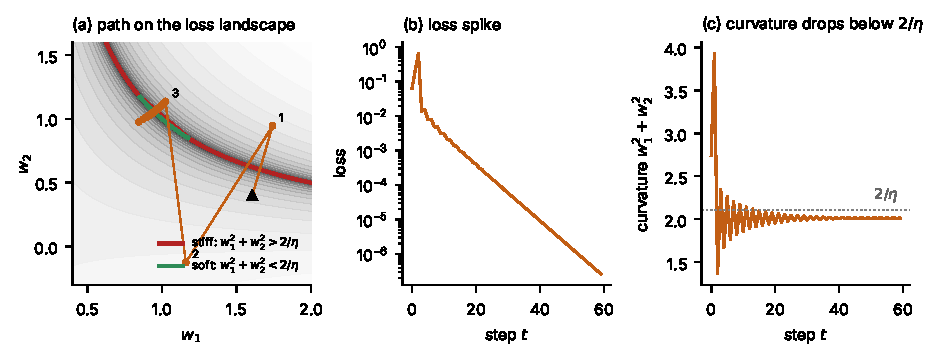
\includegraphics[width=0.62\textwidth]{figs/catapult.pdf}
\caption{A loss spike in two parameters. Gradient descent on $(uv-1)^2/2$ with $\eta=0.95$, started near $(u,v)=(1.6,0.4)$ where the curvature of the valley of minima, $u^2+v^2=2.74$, exceeds $2/\eta=2.11$. (a) The loss jumps from 0.064 to 0.66 and then decays. (b) The curvature oscillates and settles at 2.01, below $2/\eta$.}
\label{fig:catapult}
\end{figure}
